\section{Theoretical Analysis}
\label{sec:theoretical analysis}
%%%%%%%%%%%%%%%%%%%%%%%%%%%%%%%%%%%%%%%%%%%%%

\subsection{Voltage rectifier}
First the current resulting from the transformer, which is considered ideal is calculated using the formula $V_2/n_2=V_1/n_1 $, thereupon, the circuit is analyzed to understand which diodes from the rectifier are on and off for each signal of current. Next, by using KVL, it is possible to define the tension on the capacitor without addressing its discharge $V_c=A cos(w.t)-(n_{diodes} \cdot V_{on}) $, being A the amplitude of the voltage after being transformed in the inductor. 

\subsection{Envelope detector}

\textbf{Capacitor discharge:}
By using KCL, it is possible to write that $i_d = i_c + i_r$ ($i_r$ being the current if the equivalent resistor of voltage regulator).
Once the capacitor is charged and because there is fluctuation due to the sinusoidal nature of the voltage coming from the rectifier, there will be a point where $i_r = -i_c$. At this point, the diodo will turn off and the capacitor will begin to discharge. This point is called $t_{off}$ and it can be calculated like $$ t_{off}=(1/w)\cdot atan(1/w/(C  \cdot  R_{v_{reg}})).$$The function that defines the discharging is calculated using a formula obtained in the lectures: $$ V_{exp}=(A-2.V_{on}).cos(w \cdot t_{off})exp(-(t-t_{off})/(CR_{v_{reg}})$$



%\begin{figure}[h!]
 %  \includegraphics[width=.5\columnwidth]{circ_inf_0.pdf}
  %  \centering
   % \caption{Circuit at t$<$0} 
    %\label{t<0}
%\end{figure}

\subsection{Voltage at the Capacitor}

The voltage at the capacitor will be the maximum between the sinusoidal function coming from the voltage rectifier and the function of the discharge.

We can decompose this voltage, $v_C$, in its DC component, $V_c$, and its AC component, $v_c$ ($V_c$ is the mean of the function and $v_c$ is the function minus $V_c$).


\subsection{Voltage Regulator}

\textbf{Output Voltage:}
The output voltage, $v_O$, will be the voltage measured in the nodes of the first and last nodes.
This voltage can be decomposed in two components: $$v_O = V_o + v_o$$

$V_o $ will be equal to number of diodos, $n_d$ times $V_{on}$.

To get $v_o$, it is used the incremental model of the diodo, where it can be replaced by a resistor $r_d$.
After using voltage dividir, one can get the following:
$$ v_o = \frac{n_d \cdot r_d}{n_d \cdot r_d + R} \cdot v_s$$

After doing this, the output voltage, $v_O$, has been calculated.





\subsection{Results and Comparisons}



The results obtained in the simulation and theoretical analysis were similar (as it can be seen in the graphics bellow):

\begin{itemize}
  \item The value of the voltage drop of the envelope detector is close
  \item The ripple's order of magnitude is the same
  \item The value of M is similar
\end{itemize}

Note that the DC component of the voltage regulator in the theoretical analysis is equal to the one obtained in the simulation because the value of $V_{on}$ used in the theoretical analysis was taken from NGSpice. 

\begin{figure}[h]
    \centering
\subfloat[Simulation Results]{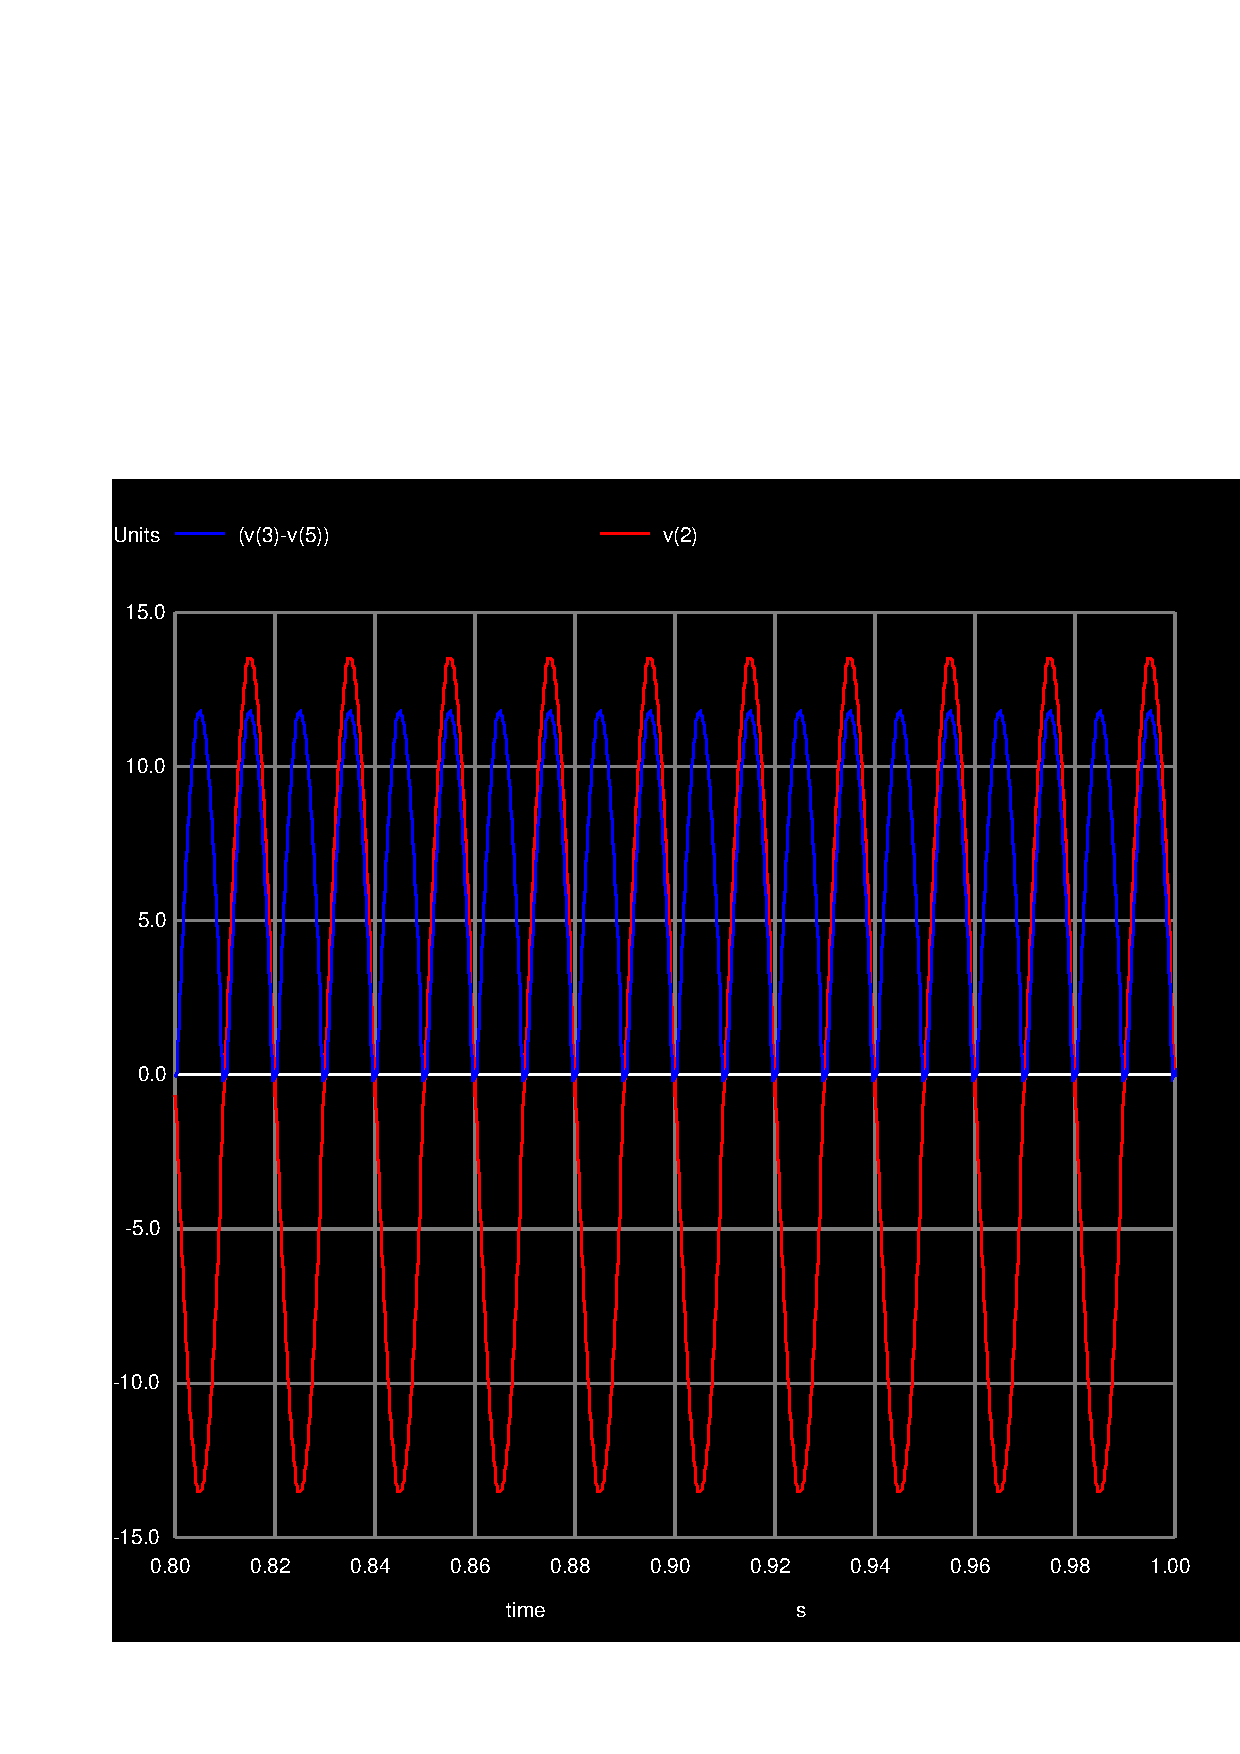
\includegraphics[width=0.40\textwidth]{../sim/outputvoltage.pdf}
\label{Fig_2_estatica}}
  \hfill
\subfloat[Theoretical Results]{\includegraphics[width=0.55\textwidth]{../mat/results_2.png}
\label{Fig_2_dinamica}}
\end{figure}

  \begin{figure}[h]
     \centering
     \caption{Envelope Detector and Voltage Regulator}
     \label{fig_2_reação_normal}
 \end{figure}


\begin{figure}[h]
    \centering
\subfloat[Simulation Results]{\includegraphics[width=0.40\textwidth]{../sim/zoom2.pdf}
\label{Fig_2_estatica}}
  \hfill
\subfloat[Theoretical Results]{\includegraphics[width=0.55\textwidth]{../mat/results.png}
\label{Fig_2_dinamica}}
\end{figure}

  \begin{figure}[h]
     \centering
     \caption{Deviation from the objective of 12 V}
     \label{fig_2_reação_normal}
 \end{figure}


\begin{table}[h]
  \centering
  \begin{tabular}{|l|r|}
    \hline    
    %{\bf Name} & {\bf Value [A or V]} \\ \hline
    \input{../sim/info}
  \end{tabular}
  \caption{Spice results. The M value and the cost were calculated by an additional octave script included in the git.}
  \label{tab:info}
\end{table}

\begin{table}[h]
  \centering
  \begin{tabular}{|l|r|}
    \hline    
    %{\bf Name} & {\bf Value [A or V]} \\ \hline
    Parameter & Value \\
\hline
Output DC level & 11.998660 V \\
\hline
Ripple & 0.009528 V \\
\hline
Cost & 64.815017 MU \\
\hline
M & 1.884083 \\
\hline

  \end{tabular}
  \caption{Spice results. The M value and the cost were calculated by an additional octave script included in the git.}
  \label{tab:info}
\end{table}


